\documentclass[bachelor, och, otchet]{SCWorks}
% параметр - тип обучения - одно из значений: spec     - специальность bachelor
%    - бакалавриат (по умолчанию) master   - магистратура параметр - форма
%    обучения - одно из значений: och   - очное (по умолчанию) zaoch - заочное
%    параметр - тип работы - одно из значений: referat    - реферат coursework -
%    курсовая работа (по умолчанию) diploma    - дипломная работа pract      -
%    отчет по практике pract      - отчет о научно-исследовательской работе
%    autoref    - автореферат выпускной работы assignment - задание на выпускную
%    квалификационную работу review     - отзыв руководителя critique   -
%    рецензия на выпускную работу параметр - включение шрифта times    -
%    включение шрифта Times New Roman (если установлен) по умолчанию выключен
\usepackage[T2A]{fontenc}
\usepackage[utf8]{inputenc}
\usepackage{graphicx}

\usepackage[sort,compress]{cite}
\usepackage{amsmath}
\usepackage{amssymb}
\usepackage{amsthm}
\usepackage{fancyvrb}
\usepackage{longtable}
\usepackage{array}
\usepackage[english,russian]{babel}
\usepackage{minted}
% Используется автором репозитория \usemintedstyle{xcode} Этот пакет включает в
%себя аналогичный Times New Roman шрифт. Необходим для успешной компиляции для
%UNIX-систем ввиду отсутствия TNR в нем. Можно использовать и для Windows.
\usepackage{tempora}
\usepackage[colorlinks=false]{hyperref}

\setminted[cpp]{fontsize=\small, breaklines=true, style=bw, linenos}
\setminted[python]{fontsize=\small, breaklines=true, style=bw, linenos}

\newcommand{\eqdef}{\stackrel {\rm def}{=}}

\newtheorem{lem}{Лемма}

% % При использовании biblatex вместо bibtex
%\usepackage[style=gost-numeric]{biblatex} \addbibresource{thesis.bib}

\begin{document}

% Кафедра (в родительном падеже)
\chair{математической кибернетики и компьютерных наук}

% Тема работы
\title{Тема работы}

% Курс
\course{2}

% Группа
\group{251}

% Факультет (в родительном падеже) (по умолчанию "факультета КНиИТ")
%\department{факультета КНиИТ}

% Специальность/направление код - наименование \napravlenie{02.03.02 "---
%Фундаментальная информатика и информационные технологии} \napravlenie{02.03.01
%"--- Математическое обеспечение и администрирование информационных систем}
%\napravlenie{09.03.01 "--- Информатика и вычислительная техника}
\napravlenie{09.03.04 "--- Программная инженерия}
%\napravlenie{10.05.01 "--- Компьютерная безопасность}

% Для студентки. Для работы студента следующая команда не нужна.
%\studenttitle{Студентки}

% Фамилия, имя, отчество в родительном падеже
\author{Иванова Ивана Ивановича}

% Заведующий кафедрой
\chtitle{доцент, к.\,ф.-м.\,н.} % степень, звание
\chname{С.\,В.\,Миронов}

%Научный руководитель (для реферата преподаватель проверяющий работу)
\satitle{доцент, к.\,ф.-м.\,н.} %должность, степень, звание
\saname{С.\,В.\,Миронов}

% Руководитель практики от организации (только для практики, для остальных типов
% работ не используется)
\patitle{к.\,ф.-м.\,н., доцент}
\paname{Д.\,Ю.\,Петров}

% Семестр (только для практики, для остальных типов работ не используется)
\term{2}

% Наименование практики (только для практики, для остальных типов работ не
% используется)
\practtype{учебная}

% Продолжительность практики (количество недель) (только для практики, для
% остальных типов работ не используется)
\duration{2}

% Даты начала и окончания практики (только для практики, для остальных типов
% работ не используется)
\practStart{01.07.2016} \practFinish{14.07.2016}

% Год выполнения отчета
\date{2021}

%\maketitle

% Включение нумерации рисунков, формул и таблиц по разделам (по умолчанию -
% нумерация сквозная) (допускается оба вида нумерации) \secNumbering


%\tableofcontents

% Раздел "Обозначения и сокращения". Может отсутствовать в работе \abbreviations
% \begin{description} \item ... "--- ... \item ... "--- ... \end{description}

% Раздел "Определения". Может отсутствовать в работе \definitions

% Раздел "Определения, обозначения и сокращения". Может отсутствовать в работе.
% Если присутствует, то заменяет собой разделы "Обозначения и сокращения" и
% "Определения" \defabbr


% Раздел "Введение"

%\intro

% После введения — серии \section, \subsection и т.д.
\section{Абстрактные синтаксические деревья}
\subsection{Управление памятью на основе регионов}
\subsubsection{Мотивировка}

Текущая реализация абстрактного синтаксического дерева имеет следующие
недостатки: 

\begin{enumerate}
    \item Выделение памяти стандартным методом может значительно фрагментировать
    оперативную память, затрудняя доступ к ней. 
    \item Любое выделение и удаление памяти требует вмешательства системных
    вызовов, что может стать причиной дополнительных издержек во время работы
    программы.
    \item Программист не имеет возможности ручного управления выделяемой им
    памятью.
\end{enumerate} 

Избавиться от этих недостатков можно используя различные оптимизации. В рамках
этой работы воспользуемся управлением памятью на основе, так называемых,
регионов (арен, зон)\cite{WangMemory}.

Под регионом далее будем понимать непрерывную область памяти, содержащую внутри
себя объекты. При запуске программы выделим регион некоторого размера, при
необходимости увеличивая его размер в некоторое постоянное число раз.

Этот подход имеет следующие преимущества:

\begin{enumerate}
    \item Элементы располагаются последовательно, в связи с чем минимизируется
    фрагментация и упрощается доступ к объектам.
    \item Выделение и освобождение памяти выполняется с минимальными издержками.
    \item Программисту предоставляется большая свобода для управления выделенной
    памятью.
\end{enumerate}

\subsubsection{Построение}
Формально определим требования к системе:
\begin{enumerate}
    \item Регион должен представлять из себя некоторый непрерывный участок
    размера $n$ байт (в начальный момент времени размер равен некоторой
    начальной величине $n_0$).
    \item При обращении к региону он должен предоставить $k$ байт памяти и
    вернуть некоторый идентификатор этого участка для последующего обращения.
    \item При заполнении региона должна быть возможность увеличить объем
    доступной памяти в некоторое число раз, которое далее будем называть
    коэффициентом увеличения.
    \item Должна быть доступна возможность эффективного освобождения всей
    выделенной регионом памяти.
\end{enumerate}

Единственной сложной операцией над регионом является его увеличение. Так как
выделение нового участка потенциально может сопровождаться изменением адресов
объектов, то необходимо организовать доступ к ним независимо от первоначального
адреса. Для этого для каждого объекта будем получать доступ к нему через
некоторый индекс.

Кроме того, коэффициент увеличения должен быть выбран таким образом, чтобы был
соблюден баланс между оптимальным объемом выделенной памяти и частотой системных
вызовов.

\subsubsection{Определение структуры}
Определим нашу структуру следующим образом:

\begin{minted}{cpp}
typedef struct arena { 
    // Указатель на начало региона 
    struct node* arena; 
    // Размер региона 
    unsigned int size; 
    // Объем выделенной регионом памяти
    unsigned int allocated; 
    } arena;
\end{minted}

\subsubsection{Инициализация}
Теперь определим функцию \verb|arena_construct|, выполняющую начальную
инициализацию состояния региона:

\begin{minted}{cpp}
int arena_construct (arena* arena) { 
    // Начальный размер региона равен некоторой постоянной, равной 
   DEFAULT_ARENA_SIZE
    arena->size = DEFAULT_ARENA_SIZE; 
    arena->allocated = 0; 
    // Выделим необходимое число памяти 
    arena->arena = malloc(sizeof(node) * DEFAULT_ARENA_SIZE); 
    // Если выделение прошло неудачно - вернем в качестве кода ошибки отличное → от 0 значение. 
    if (arena->arena == NULL) { 
        return (!0); 
    } 
    return 0; 
}
\end{minted}

\subsubsection{Выделение памяти}
После выделения некоторого объема памяти возможно обращение к ней. Определим это
обращение с помощью функции \verb|arena_allocate|:

\begin{minted}{cpp}
int arena_allocate (arena* arena, unsigned int count) { 
    // Если места в регионе недостаточно 
    if (arena->allocated + count >= arena->size) { 
        // Определим новый размер региона 
        unsigned int newSize = MULTIPLY_FACTOR * arena->size;
        // Выделим регион большего размера и освободим ранее занятую память node*
        newArena = realloc(arena->arena, newSize * sizeof(node)); 
        if (NULL == newArena) { 
            return -1; 
        } 
        arena->arena = newArena; 
        arena->size = newSize; 
        }
    // В качестве результата вернем индекс первого свободного участка региона
    unsigned int result = arena->allocated; 
    // Сместим индекс на объем выделенной памяти 
    arena->allocated += count; 
    // Вернем результат 
    return result; 
}
\end{minted}

Отметим, что наиболее часто значением \verb|MULTIPLY_FACTOR| оказывается числа
$1.5$ и $2$. Это позволяет достичь амортизационно константного времени
выполнения операции выделения памяти\cite{FacebookDoc}.

\subsubsection{Освобождение выделенной памяти}
Наконец, реализуем освобождение выделенной региону памяти с помощью функции
\verb|arena_free|

\begin{minted}{cpp}
void arena_free (arena* arena) { if (arena->arena != NULL) free(arena->arena);
    arena->arena = NULL; }
\end{minted}

\subsubsection{Модификация абстрактного синтаксического дерева}
Осталось изменить исходный код программы, чтобы обеспечить выделение памяти с
помощью полученной нами структуры данных.

Для этого воспользуемся директивой \verb|%param| и заявим в качестве параметра
переменную типа \verb|arena*|. В функциях \verb|eval|, \verb|newnum|,
\verb|newast| внесем изменения, чтобы обеспечить выделение памятью с помощью
написанных ранее
функций.

С полным кодом программы можно ознакомиться в приложении А.

\subsubsection{Сборка проекта}
Теперь проект можно собрать, незначительно изменив \verb|Makefile|:

\begin{minted}[fontsize=\small, breaklines=true, style=bw, linenos]{shell}
calc.out: calc.l calc.y arena_ast.h bison -d calc.y flex calc.l cc -o $@
    calc.tab.c lex.yy.c arena_ast.c arena.
\end{minted}
и запустить. Результат работы программы представлен на рис. 1

\begin{figure}[hbt!]
    \centering
    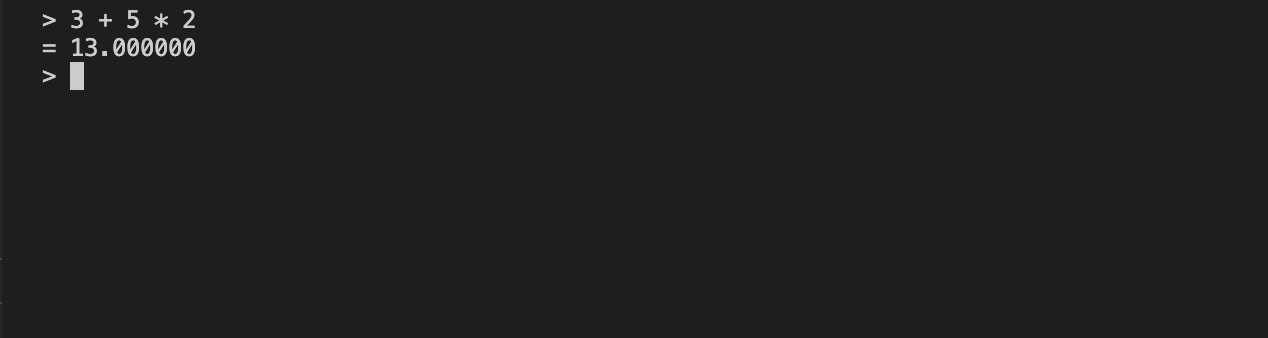
\includegraphics[scale=0.5]{naivetest.png}
    \caption{Демонстрация работы программы}
    \label{fig:naivetest}
\end{figure}

\section{Сравнение полученных реализаций}
Проведем анализ производительности полученных версий анализатора. В качестве
данных для тестирования возьмем выражения вида $\underbrace{2 + 2 + 2 \dots + 2}_{n}$ для $n =
1\dots100$ с шагом $1$. Для вычисления времени выполнения воспользуемся
библиотекой \verb|time| Python 3.9.5. Автоматизацию обеспечим с помощью
библиотеки \verb|subprocess|. Получим следующий код:

\inputminted{python}{test.py}

Кроме того, отметим, что в ранее написанные программы были внесены некоторые изменения для проведения эксперимента. Ознакомиться с ними можно в приложении А.

Ознакомиться с полным исходным кодом программы, осуществляющей
исследование производительности можно в приложении Б.

Для большей наглядности графики интерполированы полиномом с помощью функции \verb|polyfit| библиотеки \verb|numpy|.

Ознакомиться с полным исходным кодом программы, осуществляющей
анализ полученных результатов можно в приложении В.

Результаты исследования изображены на рис. 2:

\begin{figure}[hbt!]
    \centering
    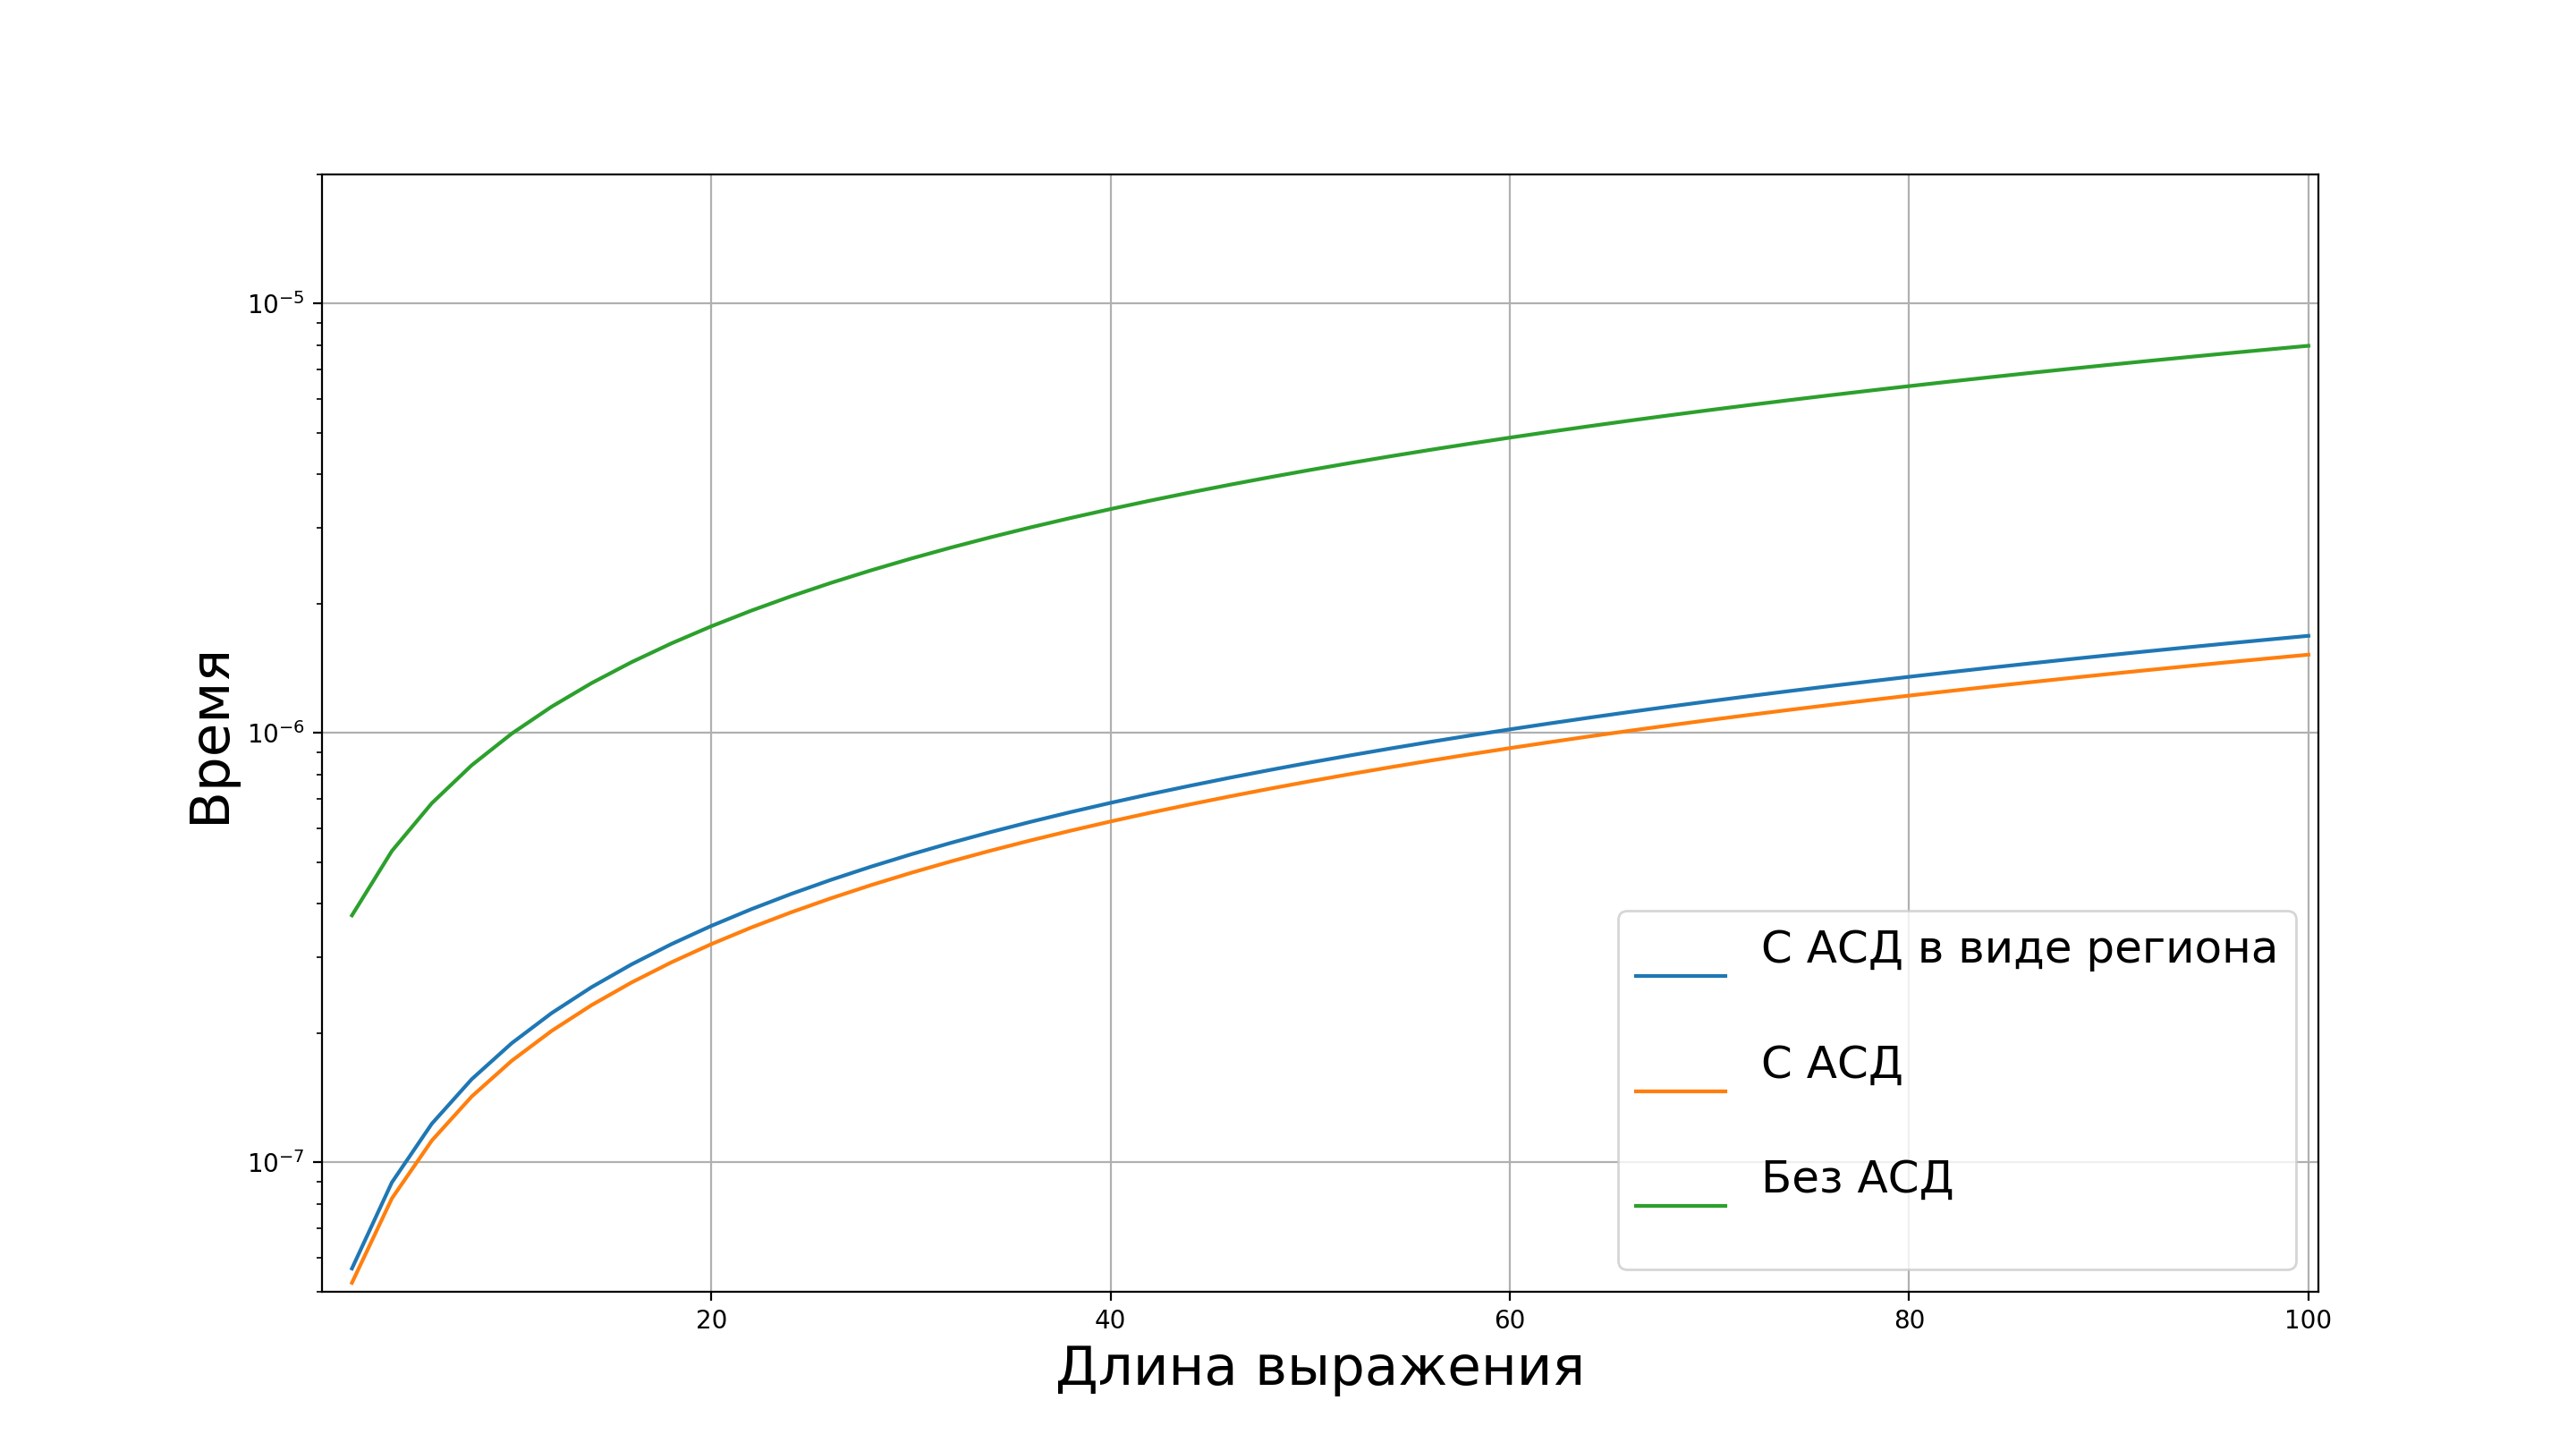
\includegraphics[scale=0.5]{benchmark.png}
    \caption{Сравнение полученных результатов}
    \label{fig:benchmark}
\end{figure}

Исследование показало, что использование абстрактных синтаксических деревьев позволяет уменьшить время работы программы более чем в $5$ раз, что существенно заметно для выражений любой длины.

Также из графиков видно, что в рамках данной работы не удалось добиться большей производительности при управлении памятью на основе регионов. Тем не менее, она все еще может считаться более предпочительной ввиду перечисленных ранее преимуществ.

% Раздел "Заключение"
\conclusion

В ходе данной работы:

\begin{enumerate}
    \item Были изучены теоретические основы построения лексических и синтаксических анализаторов.
    \item Проанализированы особенности реализации лексических и синтаксических анализаторов.
    \item Были изучены принципы работы генераторов лексического и синтаксического анализа на примере Flex и GNU Bison.
    \item Были созданы лексический и синтаксический анализаторы для анализа математического выражения.
    \item Было изучено понятие абстрактного синтаксического дерева.
    \item Проведен анализ производительности полученных реализаций.
\end{enumerate}

Таким образом, все поставленные в рамках работы задачи выполнены.

Результаты исследования показали, что абстрактные синтаксические деревья позволяют добиться увеличения производительности в $5$--$6$ раз.

А это, в свою очередь, позволяет утверждать о том, что концепция абстрактных синтаксических деревьев является крайне важной в информатике и ее приложениях, в частности, при создании синтаксических анализаторов.

%Библиографический список, составленный вручную, без использования BibTeX
%
%\begin{thebibliography}{99} \bibitem{Ione} Источник 1. \bibitem{Itwo} Источник
%  2 \end{thebibliography}

%Библиографический список, составленный с помощью BibTeX
%

\inputencoding{cp1251}
\bibliographystyle{gost780uv}
\bibliography{thesis}
\inputencoding{utf8}

% % При использовании biblatex вместо bibtex \printbibliography

% Окончание основного документа и начало приложений Каждая последующая секция
% документа будет являться приложением
\appendix 

\section{Flash-носитель с исходным кодом программ, использующихся в работе}
\noindent \textbf{Папка} \verb|src| содержит оригинальный исходный код программы:

\textbf{Папка} \verb|naive| — реализация без АСД

\textbf{Папка} \verb|naiveast| — реализация с АСД

\textbf{Папка} \verb|arena| — реализация с АСД на основе региона

\noindent \textbf{Папка} \verb|extsrc| содержит измененный исходный код, необходимый для исследования производительности:

\textbf{Папка} \verb|naive| — реализация без АСД

\textbf{Папка} \verb|naiveast| — реализация с АСД

\textbf{Папка} \verb|arena| — реализация с АСД на основе региона


\section{Исходный код программы на Python, осуществляющей исследование производительности полученных реализаций}

\inputminted{python}{test.py}

\section{Исходный код программы на Python, осуществляющей анализ
полученных результатов}

\inputminted{python}{graph.py}

\end{document}